\section{Chain of Trust}
\label{sec:20:chain_of_trust}
Signatures of real humans differ because humans do not work entirely
deterministic. The process of forging signatures of other humans requires
dictations and practice by the forger because the human factor introduces
entropy to the process of signing. On the contrary, computers are built to work
deterministically. If the same input data is processed the same way, computers
working as intended by humans produce the same output. It is, therefore, that
authentication in the digital realm is implemented through cryptography and the
knowledge of secrets. Communication involves at least two parties, which we want
to call Alice and Bob in the following example.\\

When referring to cryptographic algorithms, a secret is called a key, and based
on the kind of keys used, we can differentiate between two kinds of
cryptographic algorithms. In symmetric algorithms, the same key is used for
encryption and decryption. Alice and Bob share thus the same secret. In
asymmetric algorithms, each of Alice and Bob maintain their secrets. These keys
have a public and a private part, respectively. Alice uses the public part of
Bob's key when they want to encrypt a message for Bob, and only Bob's private
key can decrypt a message in this way.\\

Digital signatures use asymmetric cryptography. Given that Alice wants to sign a
message so that Bob can verify that Alice is the sender, both proceed as follows
to fulfill their goal. First, Alice creates a pair of keys, a public and a
private one. Alice uses their private key to sign a message and distributes
their public key so others can use it to verify Alice's signature. To create
their signature, Alice first generates a pair of keys. Alice then published
their public key to make it available to Bob. When sending a message to Bob,
Alice uses a signing function that takes the message and the private key as
input and produces a signature, which Alice sends along the message to Bob.
Knowing Alice's public key, Bob can now check the validity of the signature with
the help of a signature validation function. This function takes the message,
the signature, and Alice's public key as input and generates the answer to
whether the message was signed with the signature.\\

Another problem arises when the network increases and Bob does not have the
chance to receive Alice's key in person. To prevent man-in-the-middle attacks,
Bob must ensure that the key they received over a network originates from Alice
and not from a malicious entity. The attack surface increases with the number of
different entities Bob wants to communicate with, as Bob needs to verify the
keys of each of their communication partner. A third party, the \gls{ca}, that
Bob trusts, can help with this. The \gls{ca}'s task is to pledge to Bob that a
certified key belongs to Alice or any other chosen entity and not a potentially
malicious third party. Bob trusts the \gls{ca} to do the keys' background check
and only deliver certificates of trusted identities. Alice first registers their
key with the \gls{ca}. The \gls{ca} own a pair of private and public keys too.
It uses these keys to cryptographically bind Alice's public key to their
identity. With this certificate, Bob can validate that a public key belongs to
Alice by validating the certificate with the \glspl{ca} public key. Alice now
delivers their public key and the certificate issued by the \gls{ca} to prove
that the key belongs to them. As long as the \gls{ca} is not malicious, Bob can
detect man-in-the-middle attacks if any malicious entity ships a key not
belonging to Alice. While all participants can create certificates for their key
with a dedicated key pair, such self-signed certificates could allow
man-in-the-middle attacks again. Hence, a trusted third party creates the
certificates.\\

\begin{figure}
    \begin{center}
        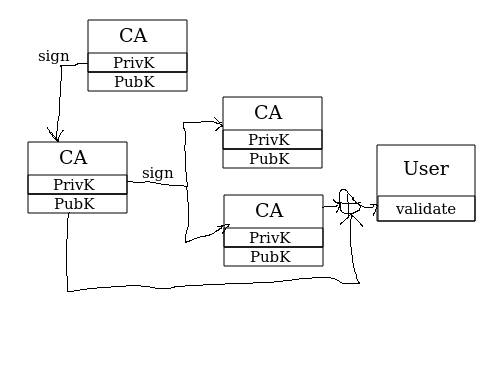
\includegraphics[width=.6\textwidth]{images/chain_of_trust_placeholder.png}
        \caption{Certifications in a chain of trust}
        \label{fig:state:technical:chain_of_trust}
    \end{center}
\end{figure}
\todo{This is a placeholder}

Because the single \gls{ca} is trusted by all participants in the network,
compromising it would mean control over all the communication in the network.
The solution to this is distributed trust. Multiple \gls{ca}'s can exist in a
network and compete with each other on the reputation gained from
users.\cite{perlman1999overview} Such a \gls{pki} is used in many network
technologies, such as HTTPS, that use the X.509 standard. Next to leaf
certificates issued to Alice and Bob, a \gls{ca} can also issue certificates on
keys that allow other entities to issue certificates and act as an \gls{ica},
creating a chain of certificates.
Figure~\ref{fig:state:technical:chain_of_trust} shows such a chain of
certificates. If Bob now wants to establish trust in the certificate provided by
Alice, they must first decide if they trust the \gls{ica}. The first step is to
verify that Alice's certificate was issued by the \gls{ica}. In the next step,
Bob needs to check all succeeding certificates until they reach the root
\gls{ca} by validating the \glspl{ica} respective certificates with the public
key of their issuer. In this way, Bob builds a chain of trust by verifying the
validity of the chain of certificates and deciding to trust the root \gls{ca}.
In the following section, we will see that such trust chains allow the
implementation of software attestation schemes.

\subsection{Remote attestation}
\label{sec:20:remote_attestation}
Remote attestation proves claims about a target
by delivering evidence to an appraiser over a network that supports these
claims. Before I further proceed to explain remote attestation, I want to
define the following terms similar to Coker et. al.\cite{coker_principles_2011}
\begin{itemize}
    \item \textbf{Appraiser}: Member of a network. Makes decisions about other
          parties on the base of delivered evidence.
    \item \textbf{Target}: Member of a network. Party about which properties the
          appraiser makes decisions.
    \item \textbf{Attestation}: Action of making claims about the target and
          delivering supportive evidence.
    \item \textbf{Measurement}: Collect evidence through direct and local
          observation
    \item \textbf{Attestation protocol}: Cryptographic protocol transmitting
          evidence about the claim. Trusted by appraiser
\end{itemize}

The appraiser and the target both follow orthogonal goals. While the appraiser
ideally wants to get as much information as possible about the target, the
target wants to preserve its privacy as well as possible and, therefore, conceal
as much information as possible. Both goals can be realized by employing a
trusted third party local to the target who can measure the target. This
third-party party then sends a signed report of the evidence on behalf of the
target. This report can contain the full raw measurement result, a reduced
variant, or a complete measurement substitute. For example, the reduced
measurement could be from a hash of the raw data. The substitute could be a
signature associated with the trusted third party that verifies that the target
fulfills the claims.

\subsection{Hardware Root of Trust}
\label{sec:20:hardware_root_of_trust}
A root of trust is defined by the Trusted Computing Group as follows:
\begin{quote}
    \textit{ A minimal set of system elements that have to be trusted because
        misbehavior is not detectable. \\
    } \mbox{ -- Trusted Computing Group\cite{tpm_architecture}}
\end{quote}

The Trusted Computing Group specifies that a hardware root of trust must be
available to enable remote attestation in a confidential computing
environment.\cite{tpm_architecture} A hardware root of trust is a device in a
computer system that the system can not manipulate. Moreover, it implements
security functionality such as encryption and random number generation. While
misbehavior is impossible to detect, hardware manufacturers can verify that
their devices work as intended by providing certificates. These certificates can
be embedded into the device with the help of tamper-resistant memory, such as
ROM or eFuses. A user can then check the validity of a certificate by consulting
the respective manufacturer's service. \\

Hardware roots of trust are necessary because system software could tamper with
software or memory to manipulate a possible software solution. The following
sections we review the most widely spread solutions to the hardware root of
trust. These implementations rely on dedicated hardware modules such as add-in
cards or unique, secure operation modes in CPU hardware. \\

\section{Trusted Execution Environments}
\label{sec:state:tee}

GlobalPlatform first used the term trusted execution environment to define a
solution for mobile trusted computing solutions.\cite{globaltee} Since then,
many definitions inconsistent and unspecific definitions have been published for
TEEs until the first precise definition was proposed by Sabt
et.al.\cite{sabt2015trusted}. They define the TEE in the following way:
\begin{quote}
    \textit{Trusted Execution Environment (TEE) is a tamper-resistant processing
        environment that runs on a separation kernel. It guarantees the authenticity of
        the executed code, the integrity of the runtime states (e.g., CPU registers,
        memory, and sensitive I/O), and the confidentiality of its code, data, and
        runtime states are stored on persistent memory. In addition, it shall be able
        to provide a remote attestation that proves its trustworthiness for third
        parties. The content of TEE is not static; it can be securely updated. The TEE
        resists all software attacks as well as physical attacks performed on the
        system's main memory. Attacks performed by exploiting backdoor security flaws
        are not possible. \\
    } \mbox{ -- Sabt et al.\cite{sabt2015trusted}}
\end{quote}

The first half of the definition describes a secure execution environment. A
secure execution environment can protect the integrity, authenticity, and
confidentiality of the application hosted by the SEE. Malicious privileged
software is thus neither able to modify the code, tamper with the runtime state,
nor observe code and data through the runtime. Contrary to TEEs, a SEE cannot
prove these claims against an appraiser, lest a third party outside the system.
This is because it does not require a root of trust to present in the system. To
prove its trustworthiness, TEEs employ remote attestation, which is the second
important aspect of the definition.\\

Trusted execution environment consists of several building blocks. The first
building block Sabt et al. propose is a secure boot. This building block allows
TEEs are used to verify that only a specific code of a particular state is
loaded. For a secure boot, a chain of trust is formed by verifying each
component's state. To generalize the secure boot requirement, a TEE must be
capable of verifying what code it loads to the environment. The second building
block is secure scheduling. Task executing in the TEE should not be able to
disrupt the main OS. Moreover, a TEE should implement means to allow
communication between the insecure world outside the TEE and the application
executing inside of it. Secure storage is one more building block. It allows the
application in the TEE to store data in a confidentiality, integrity, and
freshness-conserving way. Trusted I/O paths secure the communication between a
TEE and its users.

\subsection{TPM}
\label{sec:20:tpm}
\todo{A lot of passive to fix here}
The \gls{tpm} is a low-cost cryptographical coprocessor that offers different
cryptographic functions, such as hash functions, asymmetric and symmetric
encryption and decryption functions, asymmetric signing and verification
functions, and key generation functions. Implementations of the \gls{tpm} follow
different versions of specifications created and managed by the \gls{tcg}
consortium.\cite{tpm_architecture} The \gls{tpm} is specified by the Trusted
Computing Group as a system component with a state separate from the host system
on which it reports. The host system cannot directly manipulate the state of the
\gls{tpm} but has to use a defined interface to interact with the \gls{tpm}. To
separate the state between the host system and the \gls{tpm}, the \gls{tpm} is
implemented using dedicated hardware, such as a processor, RAM, ROM, and Flash
memory, all physically protected from the host system. Other physical separation
means can be used to implement \gls{tpm} services, such as unique processor
modes with dedicated memory access rights.\\

The most recent version of the \gls{tpm} specification is 2.0. The first
widespread family of \glspl{tpm} followed specification version 1.2, which was
implemented on modules shipped with personal computers beginning from the year
2005.\cite{arthur2015practical} One major drawback of version 1.2 was the
hard-coded usage of SHA-1 as a hashing algorithm. SHA-1 was first broken in 2005
by Wang et al.\cite{wang2005collision}. In 2011, NIST deprecated SHA-1 because
of security concerns.\cite{nist-sha1} \gls{tpm} 1.2 is constrained with respect
to its data structures to use either RSA or SHA-1\cite{tpm_architecture}
Therefore, when designing \gls{tpm} 2.0, the \gls{tcg} decided to leave the
exact algorithms specific \glspl{tpm} support open for their implementation.
Instead, the specification mandates a \gls{tpm} of version 2.0 to implement at
least one symmetric hashing, one symmetric encryption, and one asymmetric
encryption and signing algorithm. \\

In x86 systems, \gls{tpm} 2.0 is widely spread today and one of Windows 11s
system requirements. Often, \gls{tpm} is not implemented as a dedicated hardware
module but as firmware \gls{tpm}. The firmware \gls{tpm} is part of the Intel
Platform Trust Technology (Intel PTT) on Intel platforms. AMD platforms use an
implementation called fTPM, which is integrated within the platform security
processor.\cite{pirker2024brief} \\

While manufacturing, a vendor burns a \gls{ek} together with a certificate in
the \gls{tpm}. The \gls{ek} can be used to identify the \gls{tpm}, and the
certificate can be used to prove that the \gls{tpm} is genuine with the help of
the vendor's public key. Moreover, the \gls{tpm} uses the \gls{ek} as an input
to its key derivation functions. With the help of these key derivation
functions, a \gls{tpm} can generate keys for other applications such as
attestation, hashing, and signing. It never uses the \gls{ek} directly to
prevent leaking it in any form. A built-in entropy collector enables the
\gls{tpm} to generate random numbers. The \gls{tpm} uses hash functions to
generate a digest of input. Next to its cryptographic properties, the advantage
of a hash function is the output's constant length independent of the input's
length. Thus, the buffer only needs to be large enough to hold the result of the
digest. Message digests are used to store data outside of the \gls{tpm} or
generate certificates of values. The \gls{tpm} uses HMACs when storing data
outside of it. HMACs allow verifying that this data was not altered and
originates from a certain entity with the signing key.\\

The \gls{tcg} specifies two roots of trust for a trusted system. Two of them can
be implemented by the \gls{tpm}. The first is the root of trust for storage. The
\gls{tpm} implements memory that is shielded from the rest of the system, and
that can only be accessed by the \gls{tpm}. The second root of trust is the root
of trust for reporting. With its signing ability, the \gls{tpm} can attest to
values stored in its memory and create certificates for a measurement chain. The
third root of trust is the root of trust for measurement. This root is formed by
the CPU that measures on behalf of the system software or firmware. The
specification describes a core root of trust for measurement as the first
instructions executed in a new chain of trust, typically the firmware. In other
words, the core root of trust is trusted software that is believed to perform
the first measurement of the system correctly.\\

Software that performs the measurements instructs the \gls{tpm} to store its
result in \gls{pcr}. \glspl{pcr} are special registers of the \gls{tpm} that only
allow the \texttt{extend} operation and only reset when resetting the system.
The \texttt{extend} operation takes the current value of the \gls{pcr} and a new
value as input, concatenates both values, and processes the result with the help
of a hash function to create a digest that reflects the current system state.
The \gls{tpm} can assist in creating a chain of trust
(see~\ref{sec:20:chain_of_trust}) with the help of \glspl{pcr}. An example of how
to use the \gls{tpm} to build up a chain of trust is given by Arthur et
al.\cite{arthur2015practical} The system software can extend a certain \gls{pcr}
for each state before transferring control to the next application. The
application can then check the respective \gls{pcr} to contain a known good
value, indicating the platform was in a known good state before the application
was launched. If so, it can continue operation. If not, the application might
terminate. The measurement can also contain data about the application to be
launched to make sure that the application's integrity is not hurt. Remote
parties can use the \gls{tpm} attestation function to determine whether a system
was in a known good state at some time. For this, the \gls{tpm} offers the
possibility to sign the content of one or more \glspl{pcr}, producing a quote.
The remote party receives the quote, the public key, and the message contents.
The remote party can validate the certificate by executing the signature
validation function. With the public key of the \gls{tpm}, a remote party can
verify that the \gls{tpm} is genuine, and the vendor pledged to do so.
\todo{Do we need information on how system software interacts with the TPM?}

\subsection{Intel SGX}
\label{sec:20:sgx}
\todo{A lot of passive to fix here}
Intel SGX is an extension in x86\_64 processors manufactured by Intel, that
allows the creation of trusted execution environments. Intel first shipped SGX
in 2015, with processors implementing the Skylake microarchitecture. While
server-grade CPUs are still implementing SGX, Intel marked SGX was deprecated in
2021 in consumer-grade CPUs, beginning from CPUs implementing the Rocket Lake
microarchitecture. Costan et al. did an extensive study of SGX in 2016 and
documented in detail how SGX works and what it's security properties
are.\cite{costan2016intel} \\

Features of SGX include the creation of enclaves. Enclaves are especially
access-protected and encrypted system memory regions, with SGX preventing direct
memory access. In the creation process, memory pages are added to the enclave
page cache (EPC) and assigned to the enclave. Once assigned to an enclave, SGX
protects the memory page from unprivileged access, which includes all access
attempts not originating from the memory-owning enclave. After the system
software adds all pages to the enclave, it is marked as initialized. For the
initialization process, system software uses privileged instructions. After the
enclave is marked initialized, no more pages can be added to the EPC, and
interaction with the enclave is only allowed by using dedicated instructions
available only in user space. The enclave code runs at the permission level of
the application from which the enclave was called. Intel equips each CPU with
unique cryptographic keys that the CPU uses to encrypt code and data placed in
the EPC. These keys reside in memory made of electronic fuses that can not be
reprogrammed. Intel programs this memory in the factory process by burning some
of the fuses. Applications using SGX services do not necessarily need to run as
a whole in an SGX enclave. Because of restrictions on the size of the enclave's
memory, only parts of the data were handed to enclaves. Again, communications
between the enclave and user applications use special CPU instructions. In cases
where applications are split into parts residing in and outside of the enclave,
an application might want to verify the identity before sharing secrets. For
this, SGX implements local attestation.\\

As mentioned, SGX implements processor instructions dedicated to managing and
interacting with enclaves. Furthermore, SGX implementations create at least a
Launch Enclave signed by Intel. Third party enclaves that are not signed by
Intel require the Launch Enclave for successful initialization. It is necessary
in all cases when SGX is used.\\

To implement software attestation, SGX uses a second enclave provided by Intel,
the Quoting Enclave. The quoting enclave is used to verify the state
of an enclave to verify. This is done by generating a report structure. This
structure contains data such as the version and launch state of the enclave and
its identity. It is generated by calling the dedicated \textbf{EREPORT}
instruction, which cryptographically binds the generated report structure to the
enclave. The generated report structure is handed to the quoting enclave for
remote attestation. The quoting enclave then uses private keys to sign the
report to attest that the report was indeed generated from the enclave in
question. A remote party can check the quoting enclave's signature to verify the
enclave's state and identity.\\

\subsection{Confidential VM Extensions}
\label{section:20:confidential_vms}
The goal of confidential Virtual machines is to protect the entire VM from the
influence of a malicious hypervisor or other privileged software. Intel and
AMD offer individual ISA extensions for their processors to host confidential
Virtual Machines. Intel calls its solution Intel TDX, while AMDs solution is
called AMD SEV-SNP.\cite{tdx_whitepaper,kaplan_amd_2020} Both solutions use the
same fundamental building blocks to achieve the goals of confidential VMs.
Misano et al. did a extensive comparison of both
technologies.\cite{misono_confidential_2024} Intel uses the SGX module for its
implementation. Additionally, to interact with a confidential VM, the CPU must
be in the dedicated CPU operation mode called SEAM mode. Memory access is only
allowed in SEAM mode to protect confidential VMs. Once in SEAM mode, the CPU
uses its VMX capabilities to host and interact with the VM. For cryptographical
features, such as signing and key generation, Intel processors utilize the
Intel Management Engine. The Intel management Engine is a coprocessor located
in the CPU package with special firmware and a separate OS that is isolated from
the remaining parts of the system\\

For SEV-SNP, AMD uses the already implemented SEV capabilities. Unlike Intel's
implementation, AMD processors do not utilize a dedicated CPU mode but extend
the existing VM control structure by fields to enable Secure Nested paging. For
cryptography, the integrated AMD Platform Security Processor, short PSP, is
used. Both solutions encrypt the VM's memory to protect the VM from being
manipulated by system software. While in Intel's implementation, each VM is
encrypted separately, AMD's implementation encrypts, once activated, the whole
memory.\\

Both solutions use the trustee's knowledge of the initial state of the VM image.
The assumption that the approach follows is that if the VM is started in a known
state and protected from manipulation by the hypervisor or other privileged
software, then the VM can be trusted in the following. To follow this approach,
a measurement of the initial VM image is created and cryptographically bound to
the respective VM instance through a message authentication code. Before the
trustee interacts with the VM, they request the VM to verify its identity. For
this, the VM requests the cryptographical hardware to sign a report. The signed
report is then handed to the trustee. The trustee trusts the implementation in
the CPU and verifies the signature of the CPU signed report. With this, the
trustee knows if the VM images were expected. In the following, both the trustee
and the VM exchange keys for further communication.\\

\subsection{ARM TrustZone}
\label{sec:20:trustzone}
As another widely spread ISA ARM dominates the mobile sector. Like x86, the ARM
architecture offers technology to allow isolated program execution. On ARM, this
technology is called ARM TrustZone. TrustZone is optional for ARM processor
implementations and slightly differs between the ARM Cortex-A application
processors and the ARM Cortex-M microcontroller-aimed processors. In the
following, we concentrate on the implementation of ARM application
processors. Pinto and Santos did an extensive survey of ARM TrustZone in 2019.
In their work, they describe technical properties of AMR TrustZone and how to
use it for the implementation of \glspl{tee} and hypervisors. Moreover they
explain technical details of Trustzone and review it's security properties
against other \glspl{tee}.\cite{pinto_demystifying_2019}\\

Conceptually, ARM TrustZone-enabled processors offer three processor operation
modes. The most privileged mode is the Secure Monitor mode or short SM mode. The
Secure Monitor mode is the mode in which the processor boots and the firmware
and Bootloader executes. The second most privileged mode is the Secure World.
This mode is intended to execute code isolated from the third and least
privileged mode, the Normal World. The Bootloader is responsible for installing
software intended to run in the Secure World. Isolation is achieved by hardware.
For example, some registers exist twice to allow fast context switches between
the Normal and Secure World. The TrustZone Address Space Controller can be used
to partition memory into regions only accessible from the Secure World and those
accessible by both worlds. Changing between worlds can be done synchronously
using the dedicated SMC (System Monitor Call) instruction or asynchronously due
to an interrupt. The SMC instruction also triggers an interrupt. These
interrupts are served by invoking the SM, which decides upon its configuration
if the interrupt received serves as an entry point to the secure world. If so,
the Secure Monitor invokes secure world code to serve the interrupt.\\

ARM TrustZone does not implement remote attestation in hardware. Such
functionality has to be implemented by the code running in the Secure World. TEE
and remote attestation functionality can be implemented by a bare metal
application or by using a trusted OS to host secure applications in the Secure
World. The first solution minimizes code size, while the second offers the
ability to host multiple applications in the Secure World. The trusted OS would
be responsible for isolating services running in the Secure World against each
other because applications running in the Secure World are not isolated from
other applications in the Secure World by hardware. Using a trusted OS brings
the downside of an increased trusted computing base compared to a bare metal
trusted application. TrustZone does not encrypt the memory of the secure
world.\\

\subsection{Security of Hardware Solutions}
All hardware solutions isolate critical functions to protect them from being
tampered with by privileged software. Because the \gls{tpm} protects only its
state, I do not consider it when comparing the other hardware solutions. All x86
solutions protect against adversaries that can tap the memory bus. These attacks
become infeasible because all three solutions encrypt the memory content of the
respective enclaves or VMs. An adversary must break the respective cryptographic
algorithms to inspect the memory content, as the processor decrypts the memory
only once loaded. While an advisory cannot read the memory content, no solutions
protect memory access patterns from recording. ARM TrustZone does not encrypt
memory, so tapping the memory bus is possible. All solutions are vulnerable to
side-channel attacks. Concerning the trusted computing base, ARM TrustZone
relies conceptually on the functionally largest software stack. All x86
solutions only rely on their respective implementation in the CPU SoC.
Privileged software or firmware running in SMM cannot access the memory of
enclaves or VMs. On the contrary, ARM TrustZone relies on the Bootloader or
firmware to install applications into the secure world. The processor's
implementation does not protect the secure world application from being
manipulated by the firmware. We could argue that ARM TrustZone's TCB is larger
than that of the x86 solutions. As a side note, the x86 is a closed source but
could be considered rather complex. The respective security processors on the
respective x86 SoCs are running a small operating system themselves, making it
hard to compare the TCB. Nevertheless, in the x86, the whole SoC implementation
is manufactured by the same vendor, which the user ultimately has to trust.
Contrary to this, in the ARM world, the user would have to trust the SoC
manufacturer and the vendors of the Bootloader, firmware, and secure world
application.\\
